% Options for packages loaded elsewhere
\PassOptionsToPackage{unicode}{hyperref}
\PassOptionsToPackage{hyphens}{url}
%
\documentclass[
  man,floatsintext]{apa6}
\usepackage{amsmath,amssymb}
\usepackage{iftex}
\ifPDFTeX
  \usepackage[T1]{fontenc}
  \usepackage[utf8]{inputenc}
  \usepackage{textcomp} % provide euro and other symbols
\else % if luatex or xetex
  \usepackage{unicode-math} % this also loads fontspec
  \defaultfontfeatures{Scale=MatchLowercase}
  \defaultfontfeatures[\rmfamily]{Ligatures=TeX,Scale=1}
\fi
\usepackage{lmodern}
\ifPDFTeX\else
  % xetex/luatex font selection
\fi
% Use upquote if available, for straight quotes in verbatim environments
\IfFileExists{upquote.sty}{\usepackage{upquote}}{}
\IfFileExists{microtype.sty}{% use microtype if available
  \usepackage[]{microtype}
  \UseMicrotypeSet[protrusion]{basicmath} % disable protrusion for tt fonts
}{}
\makeatletter
\@ifundefined{KOMAClassName}{% if non-KOMA class
  \IfFileExists{parskip.sty}{%
    \usepackage{parskip}
  }{% else
    \setlength{\parindent}{0pt}
    \setlength{\parskip}{6pt plus 2pt minus 1pt}}
}{% if KOMA class
  \KOMAoptions{parskip=half}}
\makeatother
\usepackage{xcolor}
\usepackage{graphicx}
\makeatletter
\def\maxwidth{\ifdim\Gin@nat@width>\linewidth\linewidth\else\Gin@nat@width\fi}
\def\maxheight{\ifdim\Gin@nat@height>\textheight\textheight\else\Gin@nat@height\fi}
\makeatother
% Scale images if necessary, so that they will not overflow the page
% margins by default, and it is still possible to overwrite the defaults
% using explicit options in \includegraphics[width, height, ...]{}
\setkeys{Gin}{width=\maxwidth,height=\maxheight,keepaspectratio}
% Set default figure placement to htbp
\makeatletter
\def\fps@figure{htbp}
\makeatother
\setlength{\emergencystretch}{3em} % prevent overfull lines
\providecommand{\tightlist}{%
  \setlength{\itemsep}{0pt}\setlength{\parskip}{0pt}}
\setcounter{secnumdepth}{-\maxdimen} % remove section numbering
% Make \paragraph and \subparagraph free-standing
\ifx\paragraph\undefined\else
  \let\oldparagraph\paragraph
  \renewcommand{\paragraph}[1]{\oldparagraph{#1}\mbox{}}
\fi
\ifx\subparagraph\undefined\else
  \let\oldsubparagraph\subparagraph
  \renewcommand{\subparagraph}[1]{\oldsubparagraph{#1}\mbox{}}
\fi
% definitions for citeproc citations
\NewDocumentCommand\citeproctext{}{}
\NewDocumentCommand\citeproc{mm}{%
  \begingroup\def\citeproctext{#2}\cite{#1}\endgroup}
\makeatletter
 % allow citations to break across lines
 \let\@cite@ofmt\@firstofone
 % avoid brackets around text for \cite:
 \def\@biblabel#1{}
 \def\@cite#1#2{{#1\if@tempswa , #2\fi}}
\makeatother
\newlength{\cslhangindent}
\setlength{\cslhangindent}{1.5em}
\newlength{\csllabelwidth}
\setlength{\csllabelwidth}{3em}
\newenvironment{CSLReferences}[2] % #1 hanging-indent, #2 entry-spacing
 {\begin{list}{}{%
  \setlength{\itemindent}{0pt}
  \setlength{\leftmargin}{0pt}
  \setlength{\parsep}{0pt}
  % turn on hanging indent if param 1 is 1
  \ifodd #1
   \setlength{\leftmargin}{\cslhangindent}
   \setlength{\itemindent}{-1\cslhangindent}
  \fi
  % set entry spacing
  \setlength{\itemsep}{#2\baselineskip}}}
 {\end{list}}
\usepackage{calc}
\newcommand{\CSLBlock}[1]{\hfill\break\parbox[t]{\linewidth}{\strut\ignorespaces#1\strut}}
\newcommand{\CSLLeftMargin}[1]{\parbox[t]{\csllabelwidth}{\strut#1\strut}}
\newcommand{\CSLRightInline}[1]{\parbox[t]{\linewidth - \csllabelwidth}{\strut#1\strut}}
\newcommand{\CSLIndent}[1]{\hspace{\cslhangindent}#1}
\ifLuaTeX
\usepackage[bidi=basic]{babel}
\else
\usepackage[bidi=default]{babel}
\fi
\babelprovide[main,import]{english}
% get rid of language-specific shorthands (see #6817):
\let\LanguageShortHands\languageshorthands
\def\languageshorthands#1{}
% Manuscript styling
\usepackage{upgreek}
\captionsetup{font=singlespacing,justification=justified}

% Table formatting
\usepackage{longtable}
\usepackage{lscape}
% \usepackage[counterclockwise]{rotating}   % Landscape page setup for large tables
\usepackage{multirow}		% Table styling
\usepackage{tabularx}		% Control Column width
\usepackage[flushleft]{threeparttable}	% Allows for three part tables with a specified notes section
\usepackage{threeparttablex}            % Lets threeparttable work with longtable

% Create new environments so endfloat can handle them
% \newenvironment{ltable}
%   {\begin{landscape}\centering\begin{threeparttable}}
%   {\end{threeparttable}\end{landscape}}
\newenvironment{lltable}{\begin{landscape}\centering\begin{ThreePartTable}}{\end{ThreePartTable}\end{landscape}}

% Enables adjusting longtable caption width to table width
% Solution found at http://golatex.de/longtable-mit-caption-so-breit-wie-die-tabelle-t15767.html
\makeatletter
\newcommand\LastLTentrywidth{1em}
\newlength\longtablewidth
\setlength{\longtablewidth}{1in}
\newcommand{\getlongtablewidth}{\begingroup \ifcsname LT@\roman{LT@tables}\endcsname \global\longtablewidth=0pt \renewcommand{\LT@entry}[2]{\global\advance\longtablewidth by ##2\relax\gdef\LastLTentrywidth{##2}}\@nameuse{LT@\roman{LT@tables}} \fi \endgroup}

% \setlength{\parindent}{0.5in}
% \setlength{\parskip}{0pt plus 0pt minus 0pt}

% Overwrite redefinition of paragraph and subparagraph by the default LaTeX template
% See https://github.com/crsh/papaja/issues/292
\makeatletter
\renewcommand{\paragraph}{\@startsection{paragraph}{4}{\parindent}%
  {0\baselineskip \@plus 0.2ex \@minus 0.2ex}%
  {-1em}%
  {\normalfont\normalsize\bfseries\itshape\typesectitle}}

\renewcommand{\subparagraph}[1]{\@startsection{subparagraph}{5}{1em}%
  {0\baselineskip \@plus 0.2ex \@minus 0.2ex}%
  {-\z@\relax}%
  {\normalfont\normalsize\itshape\hspace{\parindent}{#1}\textit{\addperi}}{\relax}}
\makeatother

\makeatletter
\usepackage{etoolbox}
\patchcmd{\maketitle}
  {\section{\normalfont\normalsize\abstractname}}
  {\section*{\normalfont\normalsize\abstractname}}
  {}{\typeout{Failed to patch abstract.}}
\patchcmd{\maketitle}
  {\section{\protect\normalfont{\@title}}}
  {\section*{\protect\normalfont{\@title}}}
  {}{\typeout{Failed to patch title.}}
\makeatother

\usepackage{xpatch}
\makeatletter
\xapptocmd\appendix
  {\xapptocmd\section
    {\addcontentsline{toc}{section}{\appendixname\ifoneappendix\else~\theappendix\fi\\: #1}}
    {}{\InnerPatchFailed}%
  }
{}{\PatchFailed}
\keywords{meta theory, theory formation, cumulative science, formal models\newline\indent Word count: 6897}
\usepackage{lineno}

\linenumbers
\usepackage{csquotes}
\ifLuaTeX
  \usepackage{selnolig}  % disable illegal ligatures
\fi
\usepackage{bookmark}
\IfFileExists{xurl.sty}{\usepackage{xurl}}{} % add URL line breaks if available
\urlstyle{same}
\hypersetup{
  pdftitle={FAIR theory: Applying Open Science Principles to the Construction and Iterative Improvement of Scientific Theories},
  pdfauthor={Caspar J. Van Lissa1, Aaron Peikert2,3, Andreas M. Brandmaier2,3,4, \& Felix D. Schönbrodt5},
  pdflang={en-EN},
  pdfkeywords={meta theory, theory formation, cumulative science, formal models},
  hidelinks,
  pdfcreator={LaTeX via pandoc}}

\title{FAIR theory: Applying Open Science Principles to the Construction and Iterative Improvement of Scientific Theories}
\author{Caspar J. Van Lissa\textsuperscript{1}, Aaron Peikert\textsuperscript{2,3}, Andreas M. Brandmaier\textsuperscript{2,3,4}, \& Felix D. Schönbrodt\textsuperscript{5}}
\date{}


\shorttitle{FAIR THEORY}

\authornote{

This is a preprint paper, generated from Git Commit \# 9c5837f3.

The authors made the following contributions. Caspar J. Van Lissa: Conceptualization, Formal Analysis, Funding acquisition, Methodology, Project administration, Software, Supervision, Writing -- original draft, Writing -- review \& editing; Aaron Peikert: Formal Analysis, Writing -- original draft, Writing -- review \& editing; Andreas M. Brandmaier: Formal Analysis, Writing -- original draft, Writing -- review \& editing; Felix D. Schönbrodt: Conceptualization, Writing -- review \& editing.

Correspondence concerning this article should be addressed to Caspar J. Van Lissa, Professor Cobbenhagenlaan 125, 5037 DB Tilburg, The Netherlands. E-mail: \href{mailto:c.j.vanlissa@tilburguniversity.edu}{\nolinkurl{c.j.vanlissa@tilburguniversity.edu}}

}

\affiliation{\vspace{0.5cm}\textsuperscript{1} Tilburg University, dept. Methodology \& Statistics\\\textsuperscript{2} Center for Lifespan Psychology, Max Planck Institute for Human Development, Berlin, Germany\\\textsuperscript{3} Max Planck UCL Centre for Computational Psychiatry and Ageing Research, Berlin, Germany\\\textsuperscript{4} Department of Psychology, MSB Medical School Berlin, Berlin, Germany\\\textsuperscript{5} Ludwig-Maximilians-Universität München, Germany}

\abstract{%
Test test.
}



\begin{document}
\maketitle

The FAIR Guiding Principles (hereafter: FAIR principles) were established to improve the reusability of research data by making them more findable, accessible, interoperable and reusable {[}REF{]} for both humans and computers.
Since their inception in 2014, scholars have demonstrated their relevance for making other information artefacts more open, such as research software (Lamprecht et al., 2019) and computational workflows (S. R. Wilkinson et al., 2024).
This paper argues that the FAIR principles can advance effective and transparent scholarly communication about theory.
To this end, we introduce ``FAIR theory'':
a digital representation of a scientific theory, compliant with the FAIR principles.
By improving the efficiency of scholarly communication, FAIR theory has the potential to foster and accelerate cumulative knowledge acquisition and ultimately advance social scientific research.

\subsection{The Need for FAIR theory}\label{the-need-for-fair-theory}

The so-called ``replication crisis'' has prompted extensive reforms in social science (Lavelle, 2021; Scheel, 2022).
Concern that undisclosed flexibility in analyses was a major factor for the abundance of non-replicable findings led to widespread adoption of open science practices like preregistration and replication (Nosek et al., 2015).
These various practices ensure transparent and repeated testing of hypotheses.
However, recent reviews show that most preregistered hypothesis tests are not supported by empirical evidence (Scheel, Schijen, \& Lakens, 2021).
Thus, increased rigor in testing has revealed that the root cause of the replication crisis is more fundamental:
Psychological theories rarely produce hypotheses that are corroborated by evidence.
Furthermore, theories are often so vague that they can accommodate findings that are mutually inconsistent,
as the theory's central claims evade falsification.

Scholars have been raising concerns about the state of theory in social science for nearly 50 years (Paul E. Meehl, 1978; Robinaugh, Haslbeck, Ryan, Fried, \& Waldorp, 2021).
Two main concerns are that, first, social scientific theories lack precision compared to theories in the physical sciences (Szollosi \& Donkin, 2021).
and clarity
In other words, social scientific theories lack \emph{formalization},
which means that they do not make very accurate predictions,
and are thus hard to falsify and difficult to understand on their own,
without either substantial interpretation or additional background knowledge.
A second concern is the lack of transparent and participative scholarly communication about psychological theory and their development over time.

Given these concerns, it is an imbalance that scientific reform initiated by the open science movement has focused primarily on improving deductive methods.
The equally critical inductive processes of theory construction and theory improvement have been largely overlooked.
The present paper restores balance by applying, for the first time,
open science principles to psychological theory.
We apply the FAIR principles to scientific theories,
introducing the concept of \emph{FAIR theory} to
facilitate transparent scholarly communication and accelerate cumulative knowledge acquisition.

\subsection{Theory and Scientific Progress}\label{theory-and-scientific-progress}

According to the \emph{empirical cycle} (de Groot, 1961),
a philosophical model of cumulative knowledge acquisition,
research ideally follows a cyclical process with two phases (Figure \ref{fig:figec}).
In the deductive phase, hypotheses derived from theory are tested on data. In the inductive phase, patterns observed in data are generalized to theoretical principles.
In this model, theories are the vehicle of scientists' understanding of phenomena.
Ideally, they are iteratively updated based on deductive testing and inductive theory construction.

\begin{figure}
\centering
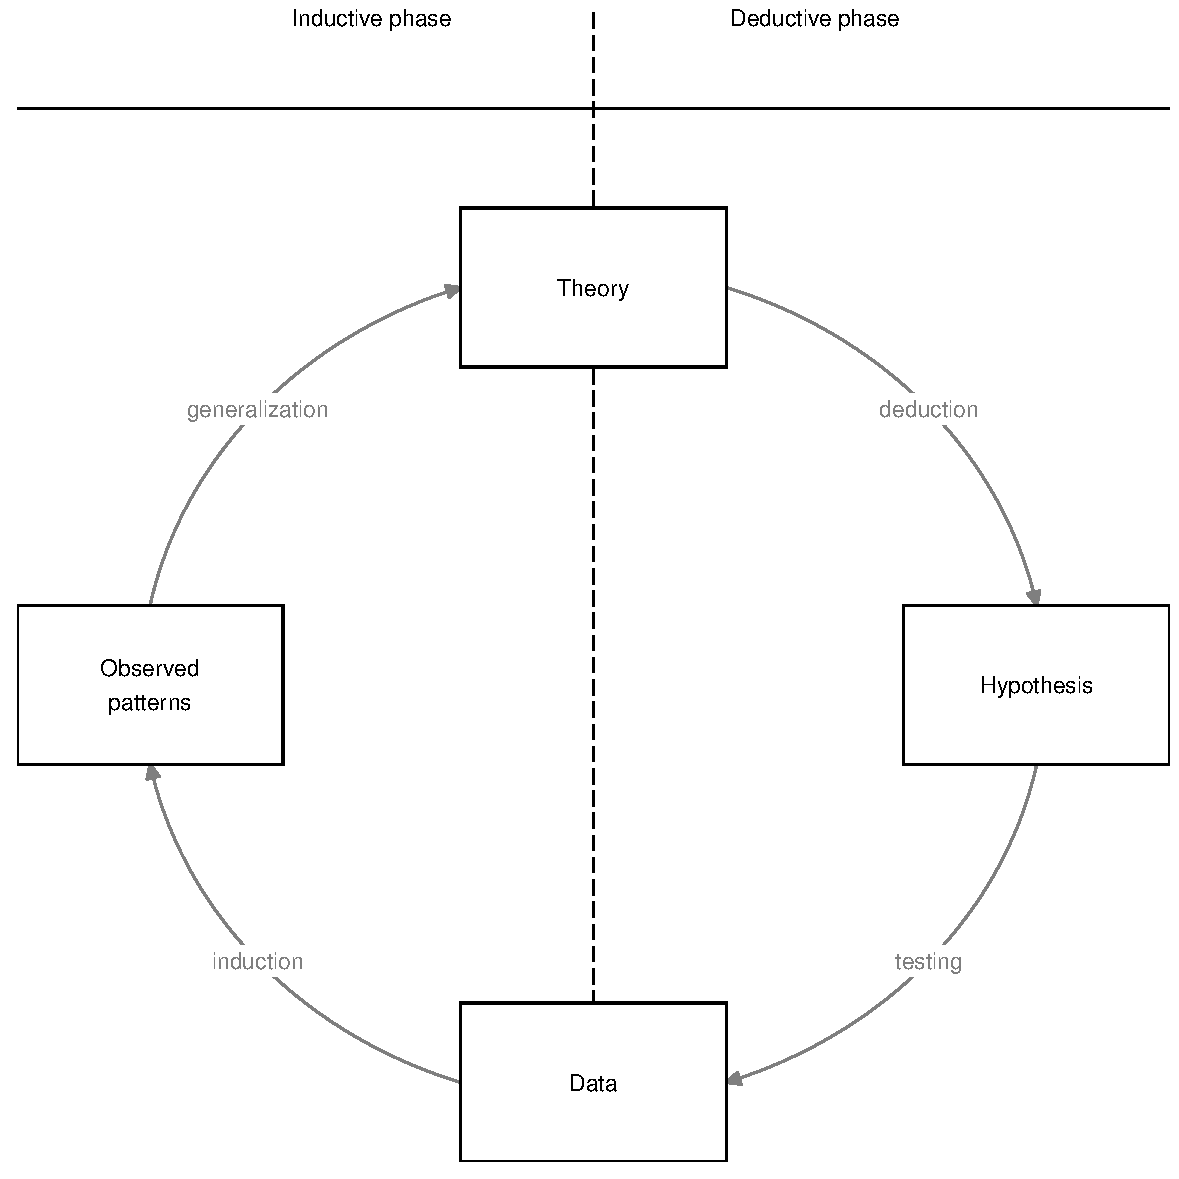
\includegraphics{empirical_cycle.pdf}
\caption{\label{fig:figec}A take on the empirical cycle by De Groot}
\end{figure}

In a progressive research program (Lakatos, 1971),
this cycle is regularly completed to iteratively advance our understanding of the studied phenomena
.
There are, however, indications that contemporary psychology falls short of this ideal.
Firstly, because hypothesis-testing research is over-represented in the literature:
According to Kühberger, Fritz, and Scherndl (2014), 89.6\% of papers published in psychology report confirmatory hypothesis tests.
Closer examination of reported deductive research reveals, however, that the link between theory and hypothesis is often tenuous (Oberauer \& Lewandowsky, 2019; Scheel, Tiokhin, Isager, \& Lakens, 2021).
Only 15\% of deductive studies referenced any theory, and theory was often not cited in relation to the hypothesis (McPhetres et al., 2021).
The remaining 85\% of deductive studies lacked an explicit derivation chain from theory to hypothesis.
In the best case, such ungrounded hypotheses are rooted in researchers' implicit theories, in which case it is particularly important to make these explicit Norouzi, Kleinberg, Vermunt, \& Van Lissa (2024).
Or, perhaps the hypotheses are not of substantive interest, such as null hypotheses that exist purely for the purpose of being rejected (Van Lissa et al., 2020), and researchers are simply testing them as part of a cultural ritual (Gigerenzer, Krauss, \& Vitouch, 2004).
Testing ad-hoc hypotheses not grounded in theory does not advance our principled understanding of psychological phenomena.
Put differently: collecting significance statements about ad-hoc hypotheses is much like trying to write novels by collecting sentences from randomly generated letter strings (van Rooij \& Baggio, 2021).

Theory thus has an uncomfortable and paradoxical role in contemporary psychology:
The majority of papers ostensibly test hypotheses,
but these are rarely derived from theory,
and test results do not routinely contribute to the improvement of existing theories.
The paradoxical role of theory in psychology is perhaps best described by Meehl's observation that theories in psychology ``lack the cumulative character of scientific knowledge. They tend neither to be refuted nor corroborated, but instead merely fade away as people lose interest'' (Paul E. Meehl, 1978).

--\textgreater{}

\subsection{Making Theory FAIR}\label{making-theory-fair}

The present paper addresses the lack of open science methods for theory development and suggests an improvement of the state of affairs by applying the FAIR principles to scientific theories.
Merely publishing theory -- as in a classic research article -- does not make it open;
to be open, theory should adhere to established open science standards.
We apply the FAIR principles to digital representations of theory,
introducing a FAIR metadata format to make theories \emph{Findable} via a DOI,
\emph{Accessible} in a machine- and human-readable filetype,
\emph{Interoperable} within the data analysis environment,
and \emph{Reusable} in the practical and legal sense, so that they may be improved over time -- at best, in a participative process.
Digital representations of theory intentionally is a broad term, particularly including textual representations of a given theory, as well as formal representations, such as mathematical notation, algorithmic pseudo code, or a set of logical clauses.
Following the original proposal of Lamprecht and colleagues,
we adapt the FAIR principles for theory, see Table \ref{tab:tabfair}.
We reflect on the necessary changes (which are minor),
as well as on the current state and future of FAIR theory in the social sciences.
The resulting principles provide guidance for instantiating theory as a FAIR information artifact,
and we provide worked examples to encourage their adoption.

\begin{lltable}

\begin{longtable}{m{.1\linewidth}m{.35\linewidth}m{.35\linewidth}m{.15\linewidth}m{.1\linewidth}m{.35\linewidth}m{.35\linewidth}m{.15\linewidth}m{.1\linewidth}m{.35\linewidth}m{.35\linewidth}m{.15\linewidth}m{.1\linewidth}m{.35\linewidth}m{.35\linewidth}m{.15\linewidth}}\noalign{\getlongtablewidth\global\LTcapwidth=\longtablewidth}
\caption{\label{tab:tabfair}}\\
\toprule
Criterion & \multicolumn{1}{c}{Original} & \multicolumn{1}{c}{Theory} & \multicolumn{1}{c}{Action}\\
\midrule
\endfirsthead
\caption*{\normalfont{Table \ref{tab:tabfair} continued}}\\
\toprule
Criterion & \multicolumn{1}{c}{Original} & \multicolumn{1}{c}{Theory} & \multicolumn{1}{c}{Action}\\
\midrule
\endhead
F1 & (Meta)data are assigned a globally unique and persistent identifier & Theory (meta)data has a global, unique and persistent identifier & Rephrased\\
F2 & Data are described with rich metadata & Theory is described with rich metadata & Rephrased\\
F3 & Metadata clearly and explicitly include the identifier of the data it describes & Metadata clearly and explicitly include identifiers for all the versions of the theory it describes & Rephrased and extended\\
F4 & (Meta)data are registered or indexed in a searchable resource & Theory and its associated metadata are included in a searchable repository & Rephrased, needs work\\
A1 & (Meta)data are retrievable by their identifier using a standardized communications protocol & Theory and its associated metadata are accessible by their identifier using a standardized communications protocol & Rephrased\\
A1.1 & The protocol is open, free, and universally implementable & The protocol is open, free, and universally implementable & Remain the same\\
A1.2 & The protocol allows for an authentication and authorization procedure, where necessary & The protocol allows for an authentication and authorization procedure, where necessary & Remain the same, but less relevant\\
A2 & Metadata are accessible, even when the data are no longer available & Theory metadata are accessible, even when the theory is no longer available & Rephrased, but less relevant\\
I1 & (Meta)data use a formal, accessible, shared, and broadly applicable language for knowledge representation & Theory and its associated metadata use a formal, accessible, shared and broadly applicable language to facilitate machine readability and reuse & Rephrased and extended\\
I2 & (Meta)data use vocabularies that follow FAIR principles & (Meta)data use vocabularies that follow FAIR principles & Rephrased\\
I2S.1 & - &  & \\
I2S.2 & - &  & \\
I3 & (Meta)data include qualified references to other (meta)data & (Meta)data includes qualified references to other (meta)data, including previous versions of the theory & Extended\\
I4S & - &  & \\
R1 & (Meta)data are richly described with a plurality of accurate and relevant attributes & Theory and its associated metadata are richly described with a plurality of accurate and relevant attributes & Rephrased\\
R1.1 & (Meta)data are released with a clear and accessible data usage license & Theory (meta)data are released with a clear and accessible license & Rephrased\\
R1.2 & (Meta)data are associated with detailed provenance & Theory (meta)data are associated with detailed provenance & Rephrased\\
R1.3 & (Meta)data meet domain-relevant community standards & Theory (meta)data and documentation meet domain-relevant community standards & Rephrased\\
\bottomrule
\end{longtable}

\end{lltable}

There are different definitions of theory,
and many of those definitions are consistent with the FAIR theory principles.
This paper defines theory as an integrated set of statements that explain phenomena consistently evidenced by patterns in data {[}bogen/woodward{]}.
Meehl (1990) provides guidance as to what kinds of ``statements'' such a theory might contain:
statements about the types of entities postulated (i.e., ontology),
statements about causal connections between those entities,
statements about the functional form of those connections,
and statements about their specific numerical values Guest (2024).

Some have defined a model as a ``specific instantiation of theory narrower in scope and often more concrete, commonly applied to a particular aspect of a given theory'' {[}REF Fried{]}.
This invites the question: if a FAIR theory is a specific instantiation of theory, how does FAIR theory differ from a model?
There is no principled difference;
theories and models derived from it exist along a continuum of specificity, where
a theory has a relatively broader scope and may contain one or more models as specific instances.
For example, following Meehl, we could envision a theory that merely specifies how specific constructs are causally connected.
From this theory, we could derive a more specific \emph{statistical model} by assuming functional form (e.g., linear effects) and error families (e.g., normal distributions).
This statistical model makes just enough assumptions to allow estimation of the remaining unknown parameters (e.g., regression slopes) from data.
Or, we could derive an even more specific \emph{generative/computational model}, which is completely parametrized (i.e., specific values of regression slopes are also assumed) such that an interpreter (e.g., the R programming language) can use the model to generate new data.
Note that broadness and narrowness are relative terms,
and one person's theory may be another person's model.
This definition also implies that FAIR models are a special case of FAIR theory.

As an applied example, consider a comprehensive theory of disease spread and pandemics which covers various psychological factors such as adherence to pandemic mitigation methods (e.g., ), pandemic-related social disruption (e.g., panic buying), or pandemic-related distress and related problems (e.g., anxiety) (Taylor, 2022).
The theory may encompass a particular transmission \emph{model} for disease spread including precise parameters for the process of infection (e.g., social distance, average duration of encounters, ventilation) and incubation times.

\subsubsection{The Role of Theory Formalization}\label{the-role-of-theory-formalization}

Concerns about the state of theory in the psychological literature revolve around two issues: theory formalization and theory (re-)use.
Greater formalization increases theories' \emph{empirical content} {[}REF{]} as it forces researchers to use precise statements, for example by specifying exact functional forms for relations or forces them to specify processes that would otherwise get away with their vague formulation in verbal theories.
For example, the phonological loop in Baddeley's verbal description of his working memory model allows at least 144 different implementations, for example, depending on how decay rate, recall success, or rehearsal sequence are precisely implemented (Lewandowsky \& Farrell, 2010).
More precise theories makes them easier to falsify,
which necessitates revising them,
thus advancing our principled understanding of the phenomena they describe.
FAIR theory does not require theories to be formal,
and formal theory can be represented in a way that is not FAIR.
It is therefore important for us to emphasize that FAIR theory imposes no restrictions on researchers regarding the manner in which theories are derived and written down.
The guidelines introduced by FAIR theory primarily pertain to how theories are documented and shared in digital environments, with the aim of enhancing their reusability and extensibility.
For example, it is possible to represent a collection of verbal propositions (perhaps derived through qualitative research) as a FAIR theory.
Conversely, a directed acyclic graph (DAG) is a type of formal theory (for example, see the empirical cycle in Figure \ref{fig:figec}),
but if it is embedded within a journal article as a bitmap image without any key words to help search engines index that article as a theory paper,
it is not FAIR.
FAIR theory is thus consistent with, but does not require, formal theory (also see \emph{Accessibility}).

\subsection{Findability}\label{findability}

Making theories Findable would allow researchers to easily identify relevant theories to inform their hypotheses,
grounding their work in established theoretical foundations.
Making theories Findable also increases the impact and reuse potential of theories across disciplines,
either through direct application (where one discipline stumbles upon a problem that is already well-understood in another discipline),
or through analogical modeling.
In analog modeling, the structure of a theory from one discipline is applied to a phenomenon in another field.
For example, predator-prey models have inspired theories of XXX, and the Eysenck model of atomic magnetism has inspired a network theory of depression.
Findability also enables meta-research on theories,
in the same way libraries and search engines have enabled scholars to study the literature via systematic reviews.
In a similar way, it would become possible to compare all theories of a specific phenomenon,
or to study structural properties of theories.

The four Findability criteria are applicable to theory with only minor adjustments, see Table \ref{tab:tabfair}.
First, this requires assigning a globally unique and persistent identifier, or DOI, to each theory (F1).
Of the many services that provide DOIs for scientific information artefacts,
Zenodo and the Open Science Framework are commonly used in psychology.
Second, Findable theory is described with rich metadata (F2).
This includes citation metadata (e.g., referencing a scientific paper that documents the theory, or a psychometric paper that operationalizes specific constructs).
It might further include domain-specific metadata, such as a reference to a taxonomy of psychological constructs (Bosco, Uggerslev, \& Steel, 2017),
ontology (Guyon, Kop, Juhel, \& Falissard, 2018),
or catalog of psychological phenomena {[}REF Noah Denny{]}.
Metadata should also include identifiers for all the versions of the theory it describes (F3);
Zenodo handles this by default by providing an overarching DOI for an information artifact which subsumes the DOIs of that artifact's versions.
Finally, these metadata should be registered or indexed in a searchable registry (F4).
This final criterion is less straightforward.
Ideally, FAIR theories should be indexed in search engines used by academics, like Google Scholar.
At present, however, these search engines are designed to index traditional print publications.
The \emph{data paper} solves this problem for research data;
the idea is that scholars publish a paper (or even preprint) as documentation for the data resource {[}REF McGIllivray on data papers{]}.
The data paper is indexed by search engines, and in turn points to the relevant information artifact.
The same solution could be applied to theories - but it seems superfluous to generate papers whose only purpose is to redirect to a specific resource.
Another solution is to manually index FAIR theories,
for example by adding them to one's Google Scholar profile,
or entering them in PURE.

At present, theories have poor findability, which impedes cumulative knowledge acquisition.
One factor contributing to theories' lack of Findability is the lack of standardized metadata, or even a standardized keyword to signal the presence of theory within a paper - terms like ``theory'', ``model'', and ``framework'' are used interchangeably.
To curb this trend, we suggest using the keyword \texttt{"FAIRtheory"} for all resources that constitute or reference a FAIR theory (separating the words \texttt{FAIR} and \texttt{theory} by a space or hyphen would lead them to be interpreted as separate tokens in many search engines.
This would allow theoretical resources to be systematically indexed, tagged, and made searchable.
Another factor contributing to the present lack of Findability is that the primary unit of dissemination and search in psychology is still the academic paper.
A paper may contain multiple resources - such as materials, data, code, and theory - but if these are not merely described in text, and not instantiated as separate informational artefacts, their findability is limited.
This would be achieved by modular publishing of theories as individually citable academic assets, with adequate metadata that is indexed in standardized repositories,
similar to the current practice of publishing empirical data in standardized repositories (e.g., DataVerse).
As with empirical data, these theories could still be connected to a specific paper which might serve as documentation and the canonical reference for the resource.

There have been notable efforts to improve theories' findability through post-hoc curation.
For example, Gray and colleagues introduced a format for representing theories,
and post many examples on their website (Gray, 2017).
Similarly, Borsboom and colleagues seek to establish a database of psychological theories {[}REF BORSBOOM{]}.
Post-hoc curation is a notable effort but does not address the root cause of the lack of Findability, however.
Ideally, Findability would be addressed ante-hoc, through documentation with rich metadata and modular publishing.

\subsection{Accessibility}\label{accessibility}

Transparent scholarly communication about theory requires that theories are accessible to all researchers and other stakeholders.
If theories are accessible, researchers can reuse and refine them,
thus accelerating cumulative knowledge acquisition.
Making theories accessible also allows stakeholders (e.g., practitioners, policy makers, advocates) to inform themselves of the current scientific understanding of specific phenomena.
While isolated empirical findings can appear fragmented and contradictory (Dumas-Mallet, Smith, Boraud, \& Gonon, 2017),
theories offer a top-down, big picture representation of the phenomena studied in a field.
In other words, theories are an important instrument in science communication.

The Accessibility criteria serve to \emph{regulate} access, not to maximize it.
These principles apply to theory with minor changes, with the caveat that there might be less of a need to restrict access to theory than there is for (human subjects) data.
Firstly, theory and its associated metadata should be accessible by their identifier using a standardized communications protocol (A1).
This can be achieved, for example, by hosting theory in a version-controlled remote repository (such as git), and archiving that repository on Zenodo for long-term storage.
The resulting resource will then have an identifier (DOI) which allows the theory to be accessed using a standardized communications protocol (download via \texttt{https} or \texttt{git}).
Secondly (A2), theory metadata should be accessible, even when the theory is no longer available,
which is also achieved via long-term storage (e.g., on Zenodo).
Git remote repositories allow for access control,
and Zenodo allows for access control of individual files/resources.
An unavailable theory typically refers to a theory that was abandoned in favor of a better or more general theory (such as the phlogiston theory, which was superseded by thermodynamics).
In general, it makes sense to keep outdated theories, in order to be able to track the genesis of theories over time, yet, we require the availability of meta data as a minimum requirement.

At present, there are several impediments to theories' accessibility.
To the extent that theories are still contained within papers,
paywalls erected by commercial publishers constitute a barrier.
Open Access publishing thus increases the accessibility of all academic output, including theory.
A second impediment is more indirect:
While open access publishing increases practical access to theories,
accessibility also requires clear and explicit communication.
This property of good theories has been dubbed ``discursive survival {[}\ldots{]}, the ability to be understood'' (Guest, 2024).
The current prevalence of strategic ambiguity renders psychological theory difficult to understand (Frankenhuis et al., 2023).
It is important to acknowledge the \emph{indeterminacy of translation} (Quine, 1970):
which holds that every communicative utterance has multiple alternative translations, with no \emph{objective} means of choosing the correct one.
It follows that an idea cannot be formalized to the point that it becomes unambiguously interpretable.
This places a theoretical upper bound on theories' ability to be understood.

Successful communication requires shared background knowledge between sender and receiver (Vogt et al., 2024).
The Kuhnian notion of ``normal science'', conducted within the context of a shared paradigm, provides shared background knowledge to facilitate mutual understanding (Kuhn, 2009).
From a pragmatic perspective, these considerations indicate that,
when striving to make theory accessible,
it is important to be as explicit as possible (e.g., about assumptions and ontological definitions),
while acknowledging that accessibility exists on a spectrum,
and that it is impossible to eliminate all ambiguity.
Rather, it may benefit scientific discourse to anticipate misunderstanding,
and use it to drive further explication of theory.
In sum, efforts to communicate theory clearly, with as few dependencies on shared background knowledge as possible, including by formalization, embedding within shared contexts, and explication of assumptions, will advance its Accessibility.

A third impediment arises when theories have a ``dependency on the author'' (DOA).
DOA occurs when a theory cannot be understood by independent scholars,
thus requiring the original author for interpretation and clarification.
We have heard DOA referred to apocryphally as the ``ask Leon'' phenomenon,
as graduate students were supposedly told to ask Leon Festinger to explain to them how their misconstrual of cognitive dissonance theory had caused their experiments to yield null results.
DOA relates to the discourse on ``Great Man Theorizing'' (Guest, 2024) because it enables gatekeeping: an author could insist that work requires their involvement or denounce work conducted outside their purview as illegitimate,
which violates checks and balances of scientific research.
DOA also renders theories immune to refutation,
because the author can claim that the theory was misconstrued when confronted with falsifying evidence, thus making it a moving target (Szollosi \& Donkin, 2021).
The fact that DOA is inherently problematic is illustrated by cases where third parties identify logical inconsistencies within a theory (e.g., Kissner, 2008).
This demonstrates that original authors are not the ultimate authority on their theories.
DOA thus unduly impedes scientific progress, and authors should make good-faith efforts to make theories as accessible as possible; both in terms of availability and in terms of interpretability.

\subsection{Interoperability}\label{interoperability}

Interoperability pertains to the property of information artefacts to ``integrate or work together {[}\ldots{]} with minimal effort'' (M. D. Wilkinson et al., 2016).
The original interoperability principles can be rephrased somewhat to apply to theory.
Firstly, theory and its associated metadata should use a formal, accessible, shared and broadly applicable language to facilitate (human- and) machine readability and reuse (I1).
The common practice of instantiating theory as lengthy prose or multi-interpretable bitmap image falls short of this ideal.
Instead, FAIR theory should, ad minimum,
be instantiated as
as a type of data that is human- and machine-readable with as few interpretative steps as possible,
as previously recommended (Van Lissa et al., 2021).
Depending on the level of formalization of the theory,
different formats may be appropriate,
such as verbal statements in plain text,
mathematical formulae,
and statements expressed in some axiomatic system.
Examples of the latter include pseudo-code,
interpretable computer code,
and Gray's theory maps (Gray, 2017).
While a theory represented as a bitmap image is not very interoperable,
the same image represented in the DOT language for representing graphs does meet this ideal.

Secondly, theory (meta)data should use vocabularies that follow FAIR principles (I2).
This is essentially a call to establish standardized ontologies,
which are themselves a type of theory (Paul E. Meehl, 1990).
Thirdly, theory (meta)data should include qualified references to other (meta)data, including previous versions of the theory (I3).
The first part of this principle allows for nested theories;
for example, a theory that specifies causal relationships between constructs could refer back to an ontological theory from which those constructs are derived.
This can be achieved by linking the DOI of those nested theories ({``Contributing {Citations} and {References},''} n.d.).
The second part of this principle allows for tracing the provenance of a theory; keeping track of its prior versions and other theories that inspired it.
This can be achieved by using Git for version control and Zenodo for archiving.

As the original definition of interoperability was somewhat narrow (M. D. Wilkinson et al., 2016),
the concept has recently been further refined in terms of facilitating ``successful communication between machines and between humans and machines'', where ``A and B are considered X-interoperable if a common operation X exists that can be applied to both'' (Vogt et al., 2024).
This definition invites the question: \emph{interoperable for what?}
Suitable answers for FAIR theory may be:
this theory is X-interoperable for deriving testable hypotheses,
or for the purpose of selecting relevant control variables,
or for the purpose of indicating the conditions necessary for observing a particular phenomenon.
This revised definition implies that theories have specific properties that incur affordances in terms of X-interoperability;
for example, Table \ref{tab:tabmeehl} illustrates the affordances of Meehl's nine properties of strong theories (properties 3-8 are grouped because they all refer to functional form).

\begin{table}[tbp]

\begin{center}
\begin{threeparttable}

\caption{\label{tab:tabmeehl}}

\begin{tabular}{ll}
\toprule
Property & \multicolumn{1}{c}{X-interoperability}\\
\midrule
1) Ontology & Variable selection\\
2) Causal connections & Model specification, covariate selection, causal inference\\
3-8) Functional Form & Deriving specific hypotheses\\
9) Numerical Value & Simulating data\\
\bottomrule
\end{tabular}

\end{threeparttable}
\end{center}

\end{table}

With regard to the state of interoperability in contemporary psychology,
Kurt Lewin's adage ``there's nothing as practical as a good theory'' (Lewin, 1943) implies that ought to be highly X-interoperable in psychological researchers' day-to-day work.
But, as we argued, this is not the case.
The examples of X-interoperability offered in Table \ref{tab:tabmeehl} illustrate that much can be gained by integrating theory directly into analysis workflows, and by making theory X-interoperable within software used for analysis.
For example, interoperable theory could be used
to select control variables for causal inference (Cinelli, Forney, \& Pearl, 2022),
or to preregister the inferential procedure that would lead to specific modifications of a theory after analyzing empirical data (Peikert, Van Lissa, \& Brandmaier, 2021),
or to derive machine-readable hypotheses (Lakens \& DeBruine, 2021) which could be automatically evaluated through integration testing (Van Lissa, 2023).
Furthermore, theories can be X-interoperable with each other to enable nesting, or using one theory to clarify elements of another theory.
For example, it should be possible to embed a theory about emotion regulation (e.g., Gross, 2015) within a theory of emotion regulation development (Morris, Silk, Steinberg, Myers, \& Robinson, 2007).

\subsection{Reusability}\label{reusability}

If take cumulative knowledge acquisition to be a goal of scientific research, then Reusability is the ultimate purpose of making theory FAIR.
Applied to FAIR theory, reusability requires that theory and its associated metadata are richly described with a plurality of accurate and relevant attributes (R1) with a clear and accessible license for reuse (R1.1), detailed provenance (R1.2), and (meta)data which meets domain-relevant community standards (R1.3).
As we will argue below, the most appropriate license for theory reuse is likely to be CC0 (no rights reserved),
although this should be combined with a culture of comprehensive (theory) citation to meet other open science requirements {[}REF TOP guidelines{]}.
Criterion R1.2 is met by version control with Git and archival on Zenodo.
Domain-relevant community standards, to a large extent, remain to be established - and this paper is the first step towards further work in that area.

If we consider the current state of Reusability in psychological theory, there appears to be a norm \emph{against} theory reuse:
\emph{``{[}Theories are{]} like toothbrushes --- no self-respecting person wants to use anyone else's''} (Mischel, 2008).
This norm impedes scientific progress.
Cumulative knowledge acquisition requires reusable theories that are continuously updated based on insights from new data (de Groot, 1961).
In our workshops on FAIR theory, we similarly notice reluctance to the notion of reusing and adapting theories,
reflected in questions such as ``who owns theory'',
and ``who determines how a theory may be reused or changed''?
These questions imply a norm against modifying theory without consent from the author reminiscent of the aforementioned problem of dependency on the author.

Licensing theories for reuse provides an unambiguous answer to such questions.
In determining what license is appropriate for theory,
it is important to consider that copyright law limits authors' rights based on the \emph{idea-expression dichotomy} (Bently, Davis, \& Ginsburg, 2010),
which holds that copyright explicitly does not
\emph{``extend to any idea, procedure, process, system, method of operation, concept, principle, or discovery''}.
Copyright may, however, extend to creative works expressing that idea (e.g., writing, visual illustrations).
It thus seems that vague, ambiguous verbal explanations of theories - in other words, those that fall short of the Accessibility criterion - are more likely to qualify for copyright protection than formal theories.
If copyright limits Reusability and does not cover ideas in their purest form (like formal theories),
then it might be counterproductive and possibly misleading to adopt a license that assumes copyright protection.
Furthermore, even if copyright would apply, academic research is covered under ``fair use'' exemptions,
so copyright would pose few restrictions to Reusability in scholarly communication.
Given these considerations, the CC0 (no rights reserved) license seems most appropriate for FAIR theory;
it explicitly waives all rights and encourages reuse.
In principle, CC0 does not require attribution.
Nevertheless, is essential that scholars do comprehensively cite theory,
including prior work that new theories are based on,
even in absence of legal obligations to do so,
to meet the definition of Reusability (R1.2, Table \ref{tab:tabfair} and to comply with other definitions of open scholarship (Aalbersberg et al., 2018).

\subsection{Additional considerations}\label{additional-considerations}

We can take inspiration from the field of computer science for well-established processes for iteratively improving information artefacts, like computer code (which we also have successfully applied in the domain of reproducible research findings, see XXX).
Using version control systems, like git, would enhance the reusability of FAIR theory by thoroughly documenting every modification in a traceable and reversible manner.
Git also facilitates diffuse and adversarial collaboration,
as independent researchers can create independent versions of existing theories through ``forking'', or suggest modifications to existing theories via ``pull requests''.
In sum, version control using Git enables systematic, collaborative, and transparent theory development,
enables studying the provenance of a theory and investigating how well different iterations of the theory explain empirical evidence (Van Lissa, 2023).

Even if scholars wish to diverge substantially from prior theory,
explicitly referring back to it enables clear comparison of the differences (Ram, 2013).

From a meta-science perspective, FAIR theory facilitates studying the state of theory in a particular subfield, and comparing theories' substantive and structural properties.

\subsubsection{Making Theories FAIR Accelerates Scientific Progress}\label{making-theories-fair-accelerates-scientific-progress}

Adopting the FAIR principles for theories can address key challenges in the current research landscape, where theories often remain isolated and underutilized. By making theories findable, accessible, interoperable, and reusable, researchers can ensure that their work is grounded in a shared, transparent, and cumulative body of knowledge. This approach enhances scholarly communication, allowing for greater scrutiny, replication, and collaboration across disciplines, ultimately leading to faster, more reliable, and more impactful scientific progress.

\section{Making a Theory FAIR}\label{making-a-theory-fair}

Open science infrastructure is an area of active development, and as such,
the approach proposed here should not be considered definitive,
but rather, as one proposal for a FAIR-compliant implementation of theory.
At the time of writing (2024), the integration of GitHub and Zenodo makes for a particularly user-friendly approach.
Nevertheless, it is important to stress that alternatives to GitHub (Gitlab, Bitbucket, etc.) and Zenodo (e.g., institutional repositories) exist.
The principles described here
(using version control and archiving major versions) could be implemented in a different workflow.

The process described here can be largely automated in R using the \texttt{theorytools} package; see the package vignette on FAIR theory, \texttt{vignette("fairtheory",\ package\ =\ "theorytools")}.

\subsection{1. Implementing the Theory}\label{implementing-the-theory}

Given that we structured our argument around the importance of FAIR theory for cumulative knowledge production through scientific research around the \emph{empirical cycle},
we decided to use it as an example for this tutorial.
Note that, while the empirical cycle is not explicitly referred to as a ``theory'' by De Groot, he derives it from ``a theory of thinking'' by Selz (REF).
We can thus consider it a meta-theory of the process of theory construction.
The empirical cycle is described on page 28 of De Groot and Spiekerman (1969):

\begin{quote}
\emph{Phase 1:} `Observation': collection and grouping of empirical materials; (tentative) formation of hypotheses.\\
\emph{Phase 2:} `Induction': formulation of hypotheses.\\
\emph{Phase 3:} `Deduction': derivation of specific consequences from the hypotheses, in the form of testable predictions.\\
\emph{Phase 4:} `Testing': of the hypotheses against new empirical materials, by way of checking whether or not the predictions are fulfilled.\\
\emph{Phase 5:} `Evaluation': of the outcome of the testing procedure with respect to the hypotheses or theories stated, as well as with a view to subsequent, continued or related, investigations.
\end{quote}

If we compare it to the levels of theory formalization (Guest \& Martin, 2021),
De Groot's theory is either at the ``theory'' or ``specification'' level.
It consists of a series of natural language statements.
We can increase the level of formalization, and present an ``implementation'' in the human- and machine-readable DOT language:

\begin{verbatim}
digraph {

  observation;
  induction;
  deduction;
  test;
  evaluation;
  
  observation -> induction;
  induction -> deduction;
  deduction -> test;
  test -> evaluation;
  evaluation -> observation;
  
}
\end{verbatim}

This language describes the model as a directed graph.
Note that the code has been organized so that the first half describes an ontology of the entities the theory postulates,
and the second half describes their proposed interrelations.
This follows the first two properties of good theory according to Meehl (Paul E. Meehl, 1990).

We can now write this implementation of the empirical cycle to a text file, say \texttt{empirical\_cycle.dot}.

\subsection{2. Creating a Project Folder}\label{creating-a-project-folder}

Create a new folder and copy the theory file from the previous step into it.
To help meet the Interoperability and Reusability criteria,
add two more files:
A README.md file with instructions for future users of your theory,
and a LICENSE file with the legal conditions for reuse.
We recommend the \texttt{CC0} license, but other options are available, see \href{https://choosealicense.com/non-software/}{https://choosealicense.com}.

\subsubsection{What's in a README?}\label{whats-in-a-readme}

The readme should contain information to help people get started with using your FAIR theory.
We suggest the following elements:

\begin{itemize}
\tightlist
\item
  Title, prefaced with \texttt{\#\ FAIR\ theory:\ The\ Theory\textquotesingle{}s\ Name}
\item
  Description: A plain-text description of the theory and its scope
\item
  Interoperability: Most README files contain a section labeled ``Getting Started'', ``Instructions'', or ``How to Use''. From a FAIR perspective, such a section might be better labeled ``Interoperability'', or ``How to Use (Interoperability)''. We propose explicitly addressing the theory's X-interoperability, telling users exactly what they can use the theory for, and how. For example, our example is implemented in the DOT language for describing graphs, so we would could provide instructions here on how to plot a DOT graph.
\item
  Contributing: Pertaining to the Reusability criterion, this section should tell users the \emph{social expectations regarding reuse and contributions}.
\item
  License: The legal complement to the preceding section, this section should refer readers to the LICENSE file to learn about the \emph{legal conditions of reuse}.
\item
  Citing this work: Tell users how to cite the theory. Note that this section is redundant with the Zenodo archive, which has a preferred citation field. The disadvantage of redundant information is that you may have to maintain this section of the README going forward. The advantage is that documenting related works in the README makes it more readily accessible to users. We suggest a compromise: to retain this section, but refer the reader to the Zenodo page.
\item
  Related works: This section should refer to the work that the FAIR theory is derived from, or documented in. Again, this is redundant with metadata entered in Zenodo (step 5). We nevertheless recommend using this section to refer to Zenodo, and/or to document one canonical reference for the theory that is unlikely to change going forward. For example, we referenced the original empirical cycle paper here:
\end{itemize}

\begin{verbatim}
This repository contains an implementation of the "empirical cycle",
a model proposed by De Groot and Spiekerman (1969, p. 28). See Zenodo for other related works.

> De Groot, A. D., & Spiekerman, J. A. A. (1969). Methodology:
Foundations of inference and research in the behavioral sciences.
De Gruyter Mouton. https://doi.org/10.1515/9783112313121
\end{verbatim}

\subsection{3. Version Control the Repository}\label{version-control-the-repository}

The field of computer science provides well-established processes for creating information artefacts that can be iteratively improved.
In particular, the practice of version control offers extensive benefits for scientific work Van Lissa et al. (2021).
To version control our project, we initiate a Git repository in the project folder.
We subsequently create a remote repository to host a copy of this local Git repository on GitHub, which will in turn be archived.
Note that the repository
must be set to ``Public'' to take advantage of GitHub's Zenodo integration.

Push the local files to the Git remote repository, and keep them synchronized going forward.

\subsection{4. Archive the Theory on Zenodo}\label{archive-the-theory-on-zenodo}

The process of archiving a GitHub repository on Zenodo is documented in a vignette in the \texttt{theorytools} R-package, so that it can be kept up-to-date.
We present a brief summary of the instructions at the time of writing here.
First, create a Zenodo account with your existing GitHub account.
Then in Zenodo, go to the GitHub section under your account.
Following the instructions on the page, activate Zenodo for your theory repository.
Then, create a new release of the GitHub repository.
You have to choose a tag and release title;
we suggest using semantic versioning for both, starting with version \texttt{0.1.0}, unless you use another convention for versioning (which should be documented in README.md).
After publishing the release,
you should be able to see the archived version in your Zenodo account,
along with a DOI.

\subsection{5. Entering Meta-Data}\label{entering-meta-data}

By default, Zenodo assumes that GitHub repositories contain software and documents them as such.
To document our archive as a FAIR theory requires adding some extra information on Zenodo.
Supplying the following information helps improve the Findability of a theory:

\begin{itemize}
\tightlist
\item
  Set the \emph{resource type} to \texttt{Model}
\item
  Verify that the \emph{title} is prefaced with \texttt{FAIR\ theory:}
\item
  Add the \emph{keyword} \texttt{fairtheory}
\item
  Optionally, submit the theory to the \href{https://zenodo.org/communities/fairtheory}{``FAIR Theory Community''} to increase its findability
\item
  List the DOIs/identifiers of \emph{related works}. Use the \texttt{Relation} field as appropriate. For example:

  \begin{itemize}
  \tightlist
  \item
    \texttt{Is\ documented\ by} can be used to reference a theory paper you wrote, in which you introduce this FAIR theory
  \item
    \texttt{Is\ derived\ from} could be used to reference a paper or book chapter that introduced an existing theory that was not previously made FAIR. We used \texttt{Is\ derived\ from} to reference De Groot and Spiekerman's empirical cycle.
  \end{itemize}
\end{itemize}

\subsection{Automating these Steps}\label{automating-these-steps}

R-users can use the \texttt{theorytools} package to partly automate the preceding steps, for example, using following code (see the package documentation for more information):

\begin{verbatim}
install.packages("theorytools")
library(theorytools)
# Use worcs to check if GitHub permissions are set:
library(worcs)
check_git()
check_github()
# Create the theory repository:
fair_theory(path = "c:/theoryfolder/empirical_cycle",
            title = "The Empirical Cycle",
            theory_file = "empirical_cycle.dot",
            remote_repo = "empirical_cycle",
            add_license = "cc0")
\end{verbatim}

Note that this function also automatically provides basic FAIR theory metadata to Zenodo.

\subsection{Comparing Implementations of a Theory}\label{comparing-implementations-of-a-theory}

As several authors have taken inspiration from the work by De Groot (de Groot, 1961),\\
we compare our interpretation of the original theory to the interpretation of others.

Subsequently, Wagenmakers and colleagues modified the theory by \emph{``{[}adding the{]} Whewell-Peirce-Reichenbach distinction between the context of discovery and the context of justification''}:

\begin{verbatim}
digraph {

  subgraph cluster_discovery {
    label="Discovery";
    hypothesis [label="New hypothesis"];
    prediction [label="New prediction"];
  }
  data  [label="Old knowledge and old data"];      
  subgraph cluster_justification {
    label="Justification";
    test [label="Test on new data"];
    evaluation;
  }

  data -> hypothesis [label="Speculate & explore"];
  hypothesis -> prediction  [label="Deduce"];
  prediction -> test  [label="Design new experiment"];
  test -> evaluation  [label="Statistical analysis"];
  evaluation -> data  [label="Knowledge accumulation"];

}
\end{verbatim}

Note, however, that there appear to be further changes:
the phases of the cycle have been renamed,
and the annotations suggest a move towards experimental empirical psychology that was absent in the original formulation.
Moreover, the label ``knowledge accumulation'' invites the question of exactly \emph{how} knowledge accumulates upon evaluation of a prior experiment.
As this lack of cumulative knowledge acquisition appears to be precisely where contemporary research practice falls short, this ambiguity invites further improvement of the theory.

Our work, too is inspired by De Groot, but our take on the empirical cycle is different again:

\begin{verbatim}
digraph {

  theory;
  prediction;
  test [label="inferential procedure"];
  observation;
  
  theory -> prediction [label="deduction"];
  prediction -> test;
  test -> observation;
  observation -> theory [label="generalization"];

}
\end{verbatim}

In our representation,
induction is not a separate phase but a mode of reasoning by which specific observations are generalized into theory.
For example, the refutation of a hypothesized effect,
or the serendipitous observation of some pattern in data,
might be a reason to revise or construct theory.
Induction, incidentally, also occurs within the link from prediction to testing:
in the form of the inductive bias of methods used to perform the test,
and auxiliary assumptions that must be made to address remaining theoretical ambiguities.

\subsection{Using FAIR theory to Perform Causal Inference}\label{using-fair-theory-to-perform-causal-inference}

Some have argued that \emph{causal explanations} are a property of good theory {[}REF Meehl, etc?{]}.
According to Pearl and colleagues,
explicit assumptions about the direction of causality allow one to perform causal inference even on cross-sectional data.
Any formal theory that is explicit about direction of causality could thus be used to guide causal inference,
and could even be integrated into the analysis environment.

In this example, we illustrate how to use DAGs for causal inference, including the detection of a violation of the initial model and subsequent adaptation of the DAG. We could use that to illustrate updating FAIR theory:

\url{https://currentprotocols.onlinelibrary.wiley.com/doi/full/10.1002/cpz1.45}

We can find more examples of causal inference with DAGs in these tutorials:

\url{https://www.r-bloggers.com/2019/08/causal-inference-with-dags-in-r/}

\url{https://www.r-bloggers.com/2018/08/applications-of-dags-in-causal-inference/}

\begin{itemize}
\tightlist
\item
  Theory is the vehicle of cumulative knowledge acquisition
\item
  According to the empirical cycle, ideally, hypotheses are derived from theory, then tested in data, and theory is amended based on the resulting insights. When this cycle is regularly completed, theories become ever more veracious representations of social scientific phenomena.
\item
  At present, there is concern over a theory crisis in the social sciences, which highlights that this system is not functioning as intended, and highlights the need for better theory.
\item
  One source of potential improvements of theory methodology that has not been previously considered is computer science.
\item
  The process of ``iteratively improving'' digital objects - in this case, computer code - is well understood.
\item
  Recent work like the FAIR software principles has demonstrated that ideals of open science apply to computer science as well.
\item
  This paper argues that, conversely, principles of computer science - particularly version control, algorithmic hypothesis generation (find better word; this is about using the digital theory object to derive implied hypotheses), and integrated testing, can also be used to improve theory methods in the social science.
\item
  We introduce ``FAIR theory'', a digital research artifact to represent formal social scientific theories
\item
  FAIR theory can be version controlled; any time new insights require modifications of the theory, these modifications can be documented in a traceable and reversable manner. Version control also enables diffuse collaboration in theory development, as other researchers can submit ``pull requests'' to suggest modifications of a theory, or can ``fork'' existing theories to create a spin-off from an existing theory.
\item
  FAIR theory allows for algorithmic derivation of hypotheses implied by the theory.
\item
  FAIR theory enables integration testing: researchers can build a ``test suite'' of evidence that must be explainable by the theory, and any modifications of the theory must also pass the test suite.
\item
  To illustrate FAIR theory's potential to accelerate cumulative knowledge acquisition, we present several tutorial examples, developed in collaboration with applied researchers across fields of social science.
\end{itemize}

\section{Discussion}\label{discussion}

\subsection{Future Directions}\label{future-directions}

One remaining issue that intersects with FAIR theory is the measurement and operationalization of psychological constructs.
Aside from the aforementioned ``theory crisis'', there has been talk of a ``measurement crisis'':
it is not always clear how theoretical constructs are operationalized, and many existing instruments have poor psychometric properties {[}REF{]}.
Additionally, the ``jingle-jangle'' fallacy is prevalent in the social sciences:
the same term is often used for distinct constructs, and conversely, different terms are used to refer to the same construct.
FAIR theory can help address the measurement crisis:
since theories can reference other theories and resources, it is possible to extend a structural theory with a theory of

FAIR theory incorporates theory into open science workflows,
facilitates scholarly communication about theories,
making it easier to share theories with less opportunity for ambiguity and misunderstanding.
FAIR Theories are easier to find, and facilitate sharing, reusing, and updating open theories.
More efficient and transparent communication about theory democratizes and accelerates cumulative knowledge acquisition,
removes barriers for knowledge exchange with the global scholarly community,
opens theory development to diverse perspectives, and enables (distributed and adversarial) collaboration.

\newpage

\section{References}\label{references}

\phantomsection\label{refs}
\begin{CSLReferences}{1}{0}
\bibitem[\citeproctext]{ref-aalbersbergMakingScienceTransparent2018}
Aalbersberg, Ij. J., Appleyard, T., Brookhart, S., Carpenter, T., Clarke, M., Curry, S., \ldots{} Vazire, S. (2018). \emph{Making {Science Transparent By Default}; {Introducing} the {TOP Statement}}. \url{https://doi.org/10.31219/osf.io/sm78t}

\bibitem[\citeproctext]{ref-bently2010copyright}
Bently, L., Davis, J., \& Ginsburg, J. C. (2010). \emph{Copyright and {Piracy}: {An} interdisciplinary critique} (Vol. 13). Cambridge University Press.

\bibitem[\citeproctext]{ref-boscoMetaBUSVehicleFacilitating2017}
Bosco, F. A., Uggerslev, K. L., \& Steel, P. (2017). {MetaBUS} as a vehicle for facilitating meta-analysis. \emph{Human Resource Management Review}, \emph{27}(1), 237--254. \url{https://doi.org/10.1016/j.hrmr.2016.09.013}

\bibitem[\citeproctext]{ref-cinelliCrashCourseGood2022}
Cinelli, C., Forney, A., \& Pearl, J. (2022). A {Crash Course} in {Good} and {Bad Controls}. \emph{Sociological Methods \& Research}, 00491241221099552. \url{https://doi.org/10.1177/00491241221099552}

\bibitem[\citeproctext]{ref-ContributingCitationsReferences}
Contributing {Citations} and {References}. (n.d.). Retrieved December 5, 2024, from \url{https://support.datacite.org/docs/data-citation}

\bibitem[\citeproctext]{ref-degrootMethodologieGrondslagenVan1961}
de Groot, A. D. (1961). \emph{Methodologie: Grondslagen van onderzoek en denken in de gedragswetenschappen}. 's Gravenhage: Uitgeverij Mouton. Retrieved from \url{https://books.google.com?id=6hiBDwAAQBAJ}

\bibitem[\citeproctext]{ref-degrootMethodologyFoundationsInference1969}
De Groot, A. D., \& Spiekerman, J. A. A. (1969). \emph{Methodology: {Foundations} of inference and research in the behavioral sciences}. De Gruyter Mouton. \url{https://doi.org/10.1515/9783112313121}

\bibitem[\citeproctext]{ref-dumas-malletPoorReplicationValidity2017}
Dumas-Mallet, E., Smith, A., Boraud, T., \& Gonon, F. (2017). Poor replication validity of biomedical association studies reported by newspapers. \emph{PLOS ONE}, \emph{12}(2), e0172650. \url{https://doi.org/10.1371/journal.pone.0172650}

\bibitem[\citeproctext]{ref-frankenhuisStrategicAmbiguitySocial2023}
Frankenhuis, W. E., Panchanathan, K., \& Smaldino, P. E. (2023). Strategic {Ambiguity} in the {Social Sciences}. \emph{Social Psychological Bulletin}, \emph{18}, 1--25. \url{https://doi.org/10.32872/spb.9923}

\bibitem[\citeproctext]{ref-friedTheoriesModelsWhat2020}
Fried, E. I. (2020). Theories and {Models}: {What They Are}, {What They Are} for, and {What They Are About}. \emph{Psychological Inquiry}, \emph{31}(4), 336--344. \url{https://doi.org/10.1080/1047840X.2020.1854011}

\bibitem[\citeproctext]{ref-gigerenzerNullRitualWhat2004}
Gigerenzer, G., Krauss, S., \& Vitouch, O. (2004). The null ritual : {What} you always wanted to know about significance testing but were afraid to ask. In D. Kaplan (Ed.), \emph{The {Sage} handbook of quantitative methodology for the social sciences} (pp. 391--408). Thousand Oaks: Sage.

\bibitem[\citeproctext]{ref-grayHowMapTheory2017}
Gray, K. (2017). How to {Map Theory}: {Reliable Methods Are Fruitless Without Rigorous Theory}. \emph{Perspectives on Psychological Science}, \emph{12}(5), 731--741. \url{https://doi.org/10.1177/1745691617691949}

\bibitem[\citeproctext]{ref-grossEmotionRegulationCurrent2015}
Gross, J. J. (2015). Emotion regulation: {Current} status and future prospects. \emph{Psychological Inquiry}, \emph{26}(1), 1--26. \url{https://doi.org/10.1080/1047840X.2014.940781}

\bibitem[\citeproctext]{ref-guestWhatMakesGood2024}
Guest, O. (2024). What {Makes} a {Good Theory}, and {How Do We Make} a {Theory Good}? \emph{Computational Brain \& Behavior}. \url{https://doi.org/10.1007/s42113-023-00193-2}

\bibitem[\citeproctext]{ref-guestHowComputationalModeling2021}
Guest, O., \& Martin, A. E. (2021). How {Computational Modeling Can Force Theory Building} in {Psychological Science}. \emph{Perspectives on Psychological Science}, \emph{16}(4), 789--802. \url{https://doi.org/10.1177/1745691620970585}

\bibitem[\citeproctext]{ref-guyonMeasurementOntologyEpistemology2018}
Guyon, H., Kop, J.-L., Juhel, J., \& Falissard, B. (2018). Measurement, ontology, and epistemology: {Psychology} needs pragmatism-realism. \emph{Theory \& Psychology}, \emph{28}(2), 149--171. \url{https://doi.org/10.1177/0959354318761606}

\bibitem[\citeproctext]{ref-kissnerIDENTIFICATIONLOGICALINCONSISTENCY2008}
Kissner, J. (2008). {ON THE IDENTIFICATION OF A LOGICAL INCONSISTENCY IN THE GENERAL THEORY OF CRIME}. \emph{Journal of Crime and Justice}. Retrieved from \url{https://www.tandfonline.com/doi/abs/10.1080/0735648X.2008.9721251}

\bibitem[\citeproctext]{ref-kuhbergerPublicationBiasPsychology2014}
Kühberger, A., Fritz, A., \& Scherndl, T. (2014). Publication {Bias} in {Psychology}: {A Diagnosis Based} on the {Correlation} between {Effect Size} and {Sample Size}. \emph{PLoS ONE}, \emph{9}(9), e105825. \url{https://doi.org/10.1371/journal.pone.0105825}

\bibitem[\citeproctext]{ref-kuhnStructureScientificRevolutions2009}
Kuhn, T. S. (2009). \emph{The structure of scientific revolutions} (3. ed., {[}Nachdr.{]}). Chicago: Univ. of Chicago Press.

\bibitem[\citeproctext]{ref-lakatosHistoryScienceIts1971}
Lakatos, I. (1971). History of {Science} and its {Rational Reconstructions}. In R. C. Buck \& R. S. Cohen (Eds.), \emph{{PSA} 1970: {In Memory} of {Rudolf Carnap Proceedings} of the 1970 {Biennial Meeting Philosophy} of {Science Association}} (pp. 91--136). Dordrecht: Springer Netherlands. \url{https://doi.org/10.1007/978-94-010-3142-4_7}

\bibitem[\citeproctext]{ref-lakensImprovingTransparencyFalsifiability2021}
Lakens, D., \& DeBruine, L. M. (2021). Improving {Transparency}, {Falsifiability}, and {Rigor} by {Making Hypothesis Tests Machine-Readable}. \emph{Advances in Methods and Practices in Psychological Science}, \emph{4}(2), 2515245920970949. \url{https://doi.org/10.1177/2515245920970949}

\bibitem[\citeproctext]{ref-lamprechtFAIRPrinciplesResearch2019}
Lamprecht, A.-L., Garcia, L., Kuzak, M., Martinez, C., Arcila, R., Martin Del Pico, E., \ldots{} Capella-Gutierrez, S. (2019). Towards {FAIR} principles for research software. \emph{Data Science}, 1--23. \url{https://doi.org/10.3233/DS-190026}

\bibitem[\citeproctext]{ref-lavelleWhenCrisisBecomes2021}
Lavelle, J. S. (2021). When a {Crisis Becomes} an {Opportunity}: {The Role} of {Replications} in {Making Better Theories}. \emph{The British Journal for the Philosophy of Science}, 714812. \url{https://doi.org/10.1086/714812}

\bibitem[\citeproctext]{ref-lewandowsky2010computational}
Lewandowsky, S., \& Farrell, S. (2010). \emph{Computational modeling in cognition: {Principles} and practice}. Sage.

\bibitem[\citeproctext]{ref-lewinPsychologyProcessGroup1943}
Lewin, K. (1943). Psychology and the {Process} of {Group Living}. \emph{The Journal of Social Psychology}, \emph{17}(1), 113--131. \url{https://doi.org/10.1080/00224545.1943.9712269}

\bibitem[\citeproctext]{ref-mcphetresDecadeTheoryReflected2021}
McPhetres, J., Albayrak-Aydemir, N., Mendes, A. B., Chow, E. C., Gonzalez-Marquez, P., Loukras, E., \ldots{} Volodko, K. (2021). A decade of theory as reflected in {Psychological Science} (2009--2019). \emph{PLOS ONE}, \emph{16}(3), e0247986. \url{https://doi.org/10.1371/journal.pone.0247986}

\bibitem[\citeproctext]{ref-meehlTheoreticalRisksTabular1978}
Meehl, Paul E. (1978). Theoretical {Risks} and {Tabular Asterisks}: {Sir Karl}, {Sir Ronald}, and the {Slow Progress} of {Soft Psychology}. \emph{Journal of Consulting \& Clinical Psychology}, \emph{46}(4), 806--834.

\bibitem[\citeproctext]{ref-meehlAppraisingAmendingTheories1990}
Meehl, Paul E. (1990). Appraising and {Amending Theories}: {The Strategy} of {Lakatosian Defense} and {Two Principles} that {Warrant It}. \emph{Psychological Inquiry}, \emph{1}(2), 108--141. \url{https://doi.org/10.1207/s15327965pli0102_1}

\bibitem[\citeproctext]{ref-mischelToothbrushProblem2008}
Mischel, W. (2008). The {Toothbrush Problem}. \emph{APS Observer}, \emph{21}. Retrieved from \url{https://www.psychologicalscience.org/observer/the-toothbrush-problem}

\bibitem[\citeproctext]{ref-morrisRoleFamilyContext2007}
Morris, A. S., Silk, J. S., Steinberg, L., Myers, S. S., \& Robinson, L. R. (2007). The role of the family context in the development of emotion regulation. \emph{Social Development}, \emph{16}(2), 361--388. \url{https://doi.org/10.1111/j.1467-9507.2007.00389.x}

\bibitem[\citeproctext]{ref-norouziCapturingCausalClaims2024}
Norouzi, R., Kleinberg, B., Vermunt, J., \& Van Lissa, C. J. (2024). \emph{Capturing {Causal Claims}: {A Fine Tuned Text Mining Model} for {Extracting Causal Sentences} from {Social Science Papers}}. Retrieved from \url{https://osf.io/kwtpm/download}

\bibitem[\citeproctext]{ref-nosekPromotingOpenResearch2015a}
Nosek, B. A., Alter, G., Banks, G. C., Borsboom, D., Bowman, S. D., Breckler, S. J., \ldots{} Yarkoni, T. (2015). Promoting an open research culture. \emph{Science}, \emph{348}(6242), 1422--1425. \url{https://doi.org/10.1126/science.aab2374}

\bibitem[\citeproctext]{ref-oberauerAddressingTheoryCrisis2019}
Oberauer, K., \& Lewandowsky, S. (2019). Addressing the theory crisis in psychology. \emph{Psychonomic Bulletin \& Review}, \emph{26}(5), 1596--1618. \url{https://doi.org/10.3758/s13423-019-01645-2}

\bibitem[\citeproctext]{ref-peikertReproducibleResearchTutorial2021}
Peikert, A., Van Lissa, C. J., \& Brandmaier, A. M. (2021). Reproducible {Research} in {R}: {A Tutorial} on {How} to {Do} the {Same Thing More Than Once}. \emph{Psych}, \emph{3}(4), 836--867. \url{https://doi.org/10.3390/psych3040053}

\bibitem[\citeproctext]{ref-quineReasonsIndeterminacyTranslation1970}
Quine, W. V. (1970). On the {Reasons} for {Indeterminacy} of {Translation}. \emph{The Journal of Philosophy}, \emph{67}(6), 178--183. \url{https://doi.org/10.2307/2023887}

\bibitem[\citeproctext]{ref-ramGitCanFacilitate2013}
Ram, K. (2013). Git can facilitate greater reproducibility and increased transparency in science. \emph{Source Code for Biology and Medicine}, \emph{8}(1), 7. \url{https://doi.org/10.1186/1751-0473-8-7}

\bibitem[\citeproctext]{ref-robinaughInvisibleHandsFine2021}
Robinaugh, D. J., Haslbeck, J. M. B., Ryan, O., Fried, E. I., \& Waldorp, L. J. (2021). Invisible {Hands} and {Fine Calipers}: {A Call} to {Use Formal Theory} as a {Toolkit} for {Theory Construction}. \emph{Perspectives on Psychological Science}, \emph{16}(4), 725--743. \url{https://doi.org/10.1177/1745691620974697}

\bibitem[\citeproctext]{ref-scheelWhyMostPsychological2022}
Scheel, A. M. (2022). Why most psychological research findings are not even wrong. \emph{Infant and Child Development}, \emph{31}(1), e2295. \url{https://doi.org/10.1002/icd.2295}

\bibitem[\citeproctext]{ref-scheelExcessPositiveResults2021}
Scheel, A. M., Schijen, M. R. M. J., \& Lakens, D. (2021). An {Excess} of {Positive Results}: {Comparing} the {Standard Psychology Literature With Registered Reports}. \emph{Advances in Methods and Practices in Psychological Science}, \emph{4}(2), 25152459211007467. \url{https://doi.org/10.1177/25152459211007467}

\bibitem[\citeproctext]{ref-scheelWhyHypothesisTesters2021}
Scheel, A. M., Tiokhin, L., Isager, P. M., \& Lakens, D. (2021). Why {Hypothesis Testers Should Spend Less Time Testing Hypotheses}. \emph{Perspectives on Psychological Science}, \emph{16}(4), 744--755. \url{https://doi.org/10.1177/1745691620966795}

\bibitem[\citeproctext]{ref-szollosiArrestedTheoryDevelopment2021}
Szollosi, A., \& Donkin, C. (2021). Arrested theory development: {The} misguided distinction between exploratory and confirmatory research. \emph{Perspectives on Psychological Science}, \emph{16}(4), 717--724. \url{https://doi.org/10.1177/1745691620966796}

\bibitem[\citeproctext]{ref-taylor2022psychology}
Taylor, S. (2022). The psychology of pandemics. \emph{Annual Review of Clinical Psychology}, \emph{18}(1), 581--609.

\bibitem[\citeproctext]{ref-vanlissaUsingEndpointsCheck2023}
Van Lissa, C. J. (2023). Using {Endpoints} to {Check Reproducibility} {[}Package Documentation{]}. Retrieved March 21, 2024, from \url{https://cjvanlissa.github.io/worcs/articles/endpoints.html}

\bibitem[\citeproctext]{ref-vanlissaWORCSWorkflowOpen2021}
Van Lissa, C. J., Brandmaier, A. M., Brinkman, L., Lamprecht, A.-L., Peikert, A., Struiksma, M. E., \& Vreede, B. M. I. (2021). {WORCS}: {A} workflow for open reproducible code in science. \emph{Data Science}, \emph{4}(1), 29--49. \url{https://doi.org/10.3233/DS-210031}

\bibitem[\citeproctext]{ref-vanlissaTeacherCornerEvaluating2020}
Van Lissa, C. J., Gu, X., Mulder, J., Rosseel, Y., Zundert, C. V., \& Hoijtink, H. (2020). Teacher's {Corner}: {Evaluating Informative Hypotheses Using} the {Bayes Factor} in {Structural Equation Models}. \emph{Structural Equation Modeling: A Multidisciplinary Journal}, \emph{0}(0), 1--10. \url{https://doi.org/10.1080/10705511.2020.1745644}

\bibitem[\citeproctext]{ref-vanrooijTheoryTestHow2021}
van Rooij, I., \& Baggio, G. (2021). Theory {Before} the {Test}: {How} to {Build High-Verisimilitude Explanatory Theories} in {Psychological Science}. \emph{Perspectives on Psychological Science}, \emph{16}(4), 682--697. \url{https://doi.org/10.1177/1745691620970604}

\bibitem[\citeproctext]{ref-vogtFAIR20Extending2024}
Vogt, L., Strömert, P., Matentzoglu, N., Karam, N., Konrad, M., Prinz, M., \& Baum, R. (2024, May 6). {FAIR} 2.0: {Extending} the {FAIR Guiding Principles} to {Address Semantic Interoperability}. Retrieved November 20, 2024, from \url{http://arxiv.org/abs/2405.03345}

\bibitem[\citeproctext]{ref-wilkinsonFAIRGuidingPrinciples2016a}
Wilkinson, M. D., Dumontier, M., Aalbersberg, Ij. J., Appleton, G., Axton, M., Baak, A., \ldots{} Mons, B. (2016). The {FAIR Guiding Principles} for scientific data management and stewardship. \emph{Scientific Data}, \emph{3}(1), 160018. \url{https://doi.org/10.1038/sdata.2016.18}

\bibitem[\citeproctext]{ref-wilkinson2024applying}
Wilkinson, S. R., Aloqalaa, M., Belhajjame, K., Crusoe, M. R., Kinoshita, B. de P., Gadelha, L., et al.others. (2024). \emph{Applying the {FAIR} principles to computational workflows}. Retrieved from \url{https://arxiv.org/abs/2410.03490}

\end{CSLReferences}


\end{document}
